\documentclass[border=2mm]{standalone}
\usepackage{amsmath}
\usepackage[dvipsnames]{xcolor}
\usepackage{tikz}
\usetikzlibrary{patterns}

\begin{document}
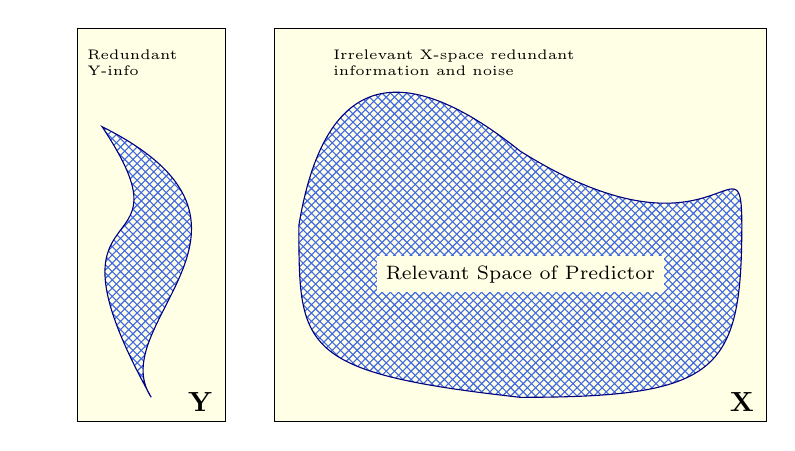
\begin{tikzpicture}[scale = 1.25]
    \begin{scope} % Response Matrix
      \draw [Black, fill=Yellow!10] (0, 0) rectangle (1.5, 4);
      \draw [NavyBlue, pattern=crosshatch, pattern color=RoyalBlue]
        (0.75, 0.25) 
            .. controls (-0.5, 2.5) and (1.25, 1.5) .. (0.25, 3) 
            .. controls (2.25, 2) and (0.25, 1) .. (0.75, 0.25);
        \node (X) at (1.25, 0.2) {$\mathbf{Y}$};
       \node [fill=Yellow!10, font=\tiny, text width = .7cm] (label) at (0.38, 3.65)
        {Redundant Y-info};
    \end{scope}
    \begin{scope}[shift={(2, 0)}] % Predictor Matrix
        \draw [Black, fill=Yellow!10] (0, 0) rectangle (5, 4);
        \draw [NavyBlue, pattern=crosshatch, pattern color=RoyalBlue]
          (2.5, 0.25) 
            .. controls (4.5, 0.25) and (4.75, 0.5) .. (4.75, 2) 
            .. controls (4.75, 3) and (4.5, 1.5) .. (2.5, 2.75)
            .. controls (1.25, 3.75) and (0.5, 3.5) .. (0.25, 2) 
            .. controls (0.25, 0.75) and (0.25, 0.5) .. (2.5, 0.25);
        \node (X) at (4.75, 0.2) {$\mathbf{X}$};
        \node [fill=Yellow!10, font=\scriptsize] (label) at (2.5, 1.5)
          {Relevant Space of Predictor};
        \node [fill=Yellow!10, font=\tiny, text width = 3.5cm] (label) at (2, 3.65)
        {Irrelevant X-space redundant information and noise};
    \end{scope}
\end{tikzpicture}
\end{document}